\documentclass[10pt,a4paper]{article}
\usepackage[utf8]{inputenc}
\usepackage[italian]{babel}
\usepackage{amsmath}
\usepackage{amsfonts}
\usepackage{amssymb}
\usepackage{graphicx}
\usepackage[left=2cm,right=2cm,top=2cm,bottom=2cm]{geometry}
\newcommand{\rem}[1]{[\emph{#1}]}

\author{Gruppo xx \\ Federico Belliardo, Francesco MAzzoncini, Giulia Franchi}
\title{Esercitazione N.5: Transistor JFET.}
\begin{document}

\maketitle

\section{Scopo e strumentazione}
Studiare le caratteristiche e realizzare un amplificatore con il JFET a canale N 2N3819.


\section{Studio funzionamento del JFET}
\paragraph{Montaggio e ossevazioni qualitative.}
E' stato montato il circuito in figura \ref{circuito1}, con  $R_1 = \pm$, $R_2 = \pm$, $V_1 = \pm $ e $V_2 = \pm$. Le due sorgenti di tensione DC ono state ottenute dalle due boccole del generatore in dotazione.

\begin{figure}
\centering
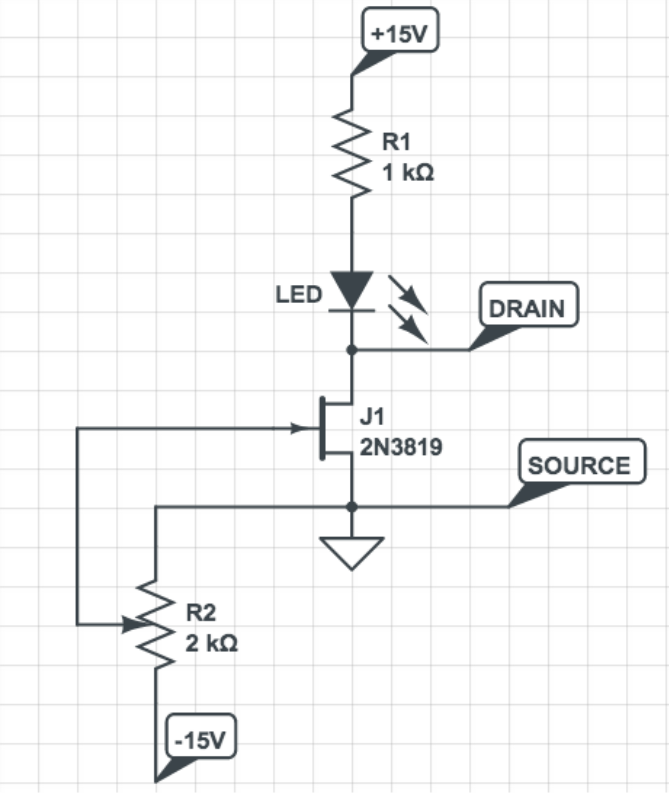
\includegraphics[scale=0.4]{circuito1.png}
\caption{Schema di JFET in corrente continua.\label{circuito1}}
\end{figure}

Variando la resistenza del potenziometro (partitore di tensione) cambia la tensione di \emph{gate} ($V_{GS}$), dunque il JFET entra in conduzione solamente quando si supera la tensione $V_{GS} > V_{P}$ (tensione di \emph{pinch-off}, quando cioò succede si accende il led. Qualitatvamente stimiamo: $V_P = \pm$.
\paragraph{Misura della corrente $I_D$ in funzione di $V_GS$.}
Si sono prese misure della tensione $V_{GS}$ e di $V_{R1}$ utilizzando il multimetro digitale, da $V_{R1}$ si è ricavata poi $I_D = \frac{V_{R1}}{R_1}$. \rem{Ne possiamo usare due di multimetri?}. Nella tabella \ref{correnteId} e in figura \ref{graficoCorrenteId} sono riporati i dati presi. \\
La retta di carico è: $V_1 - R_1 I_D-V_{\gamma}-V_{DS} = 0$ quando scorre corrente $I_D$ (cioè sono in zona ohmica o di saturazione), mentre $V_{DS} = V_1$ quando sono in zona di interdizione.\\
\begin{figure}
\centering
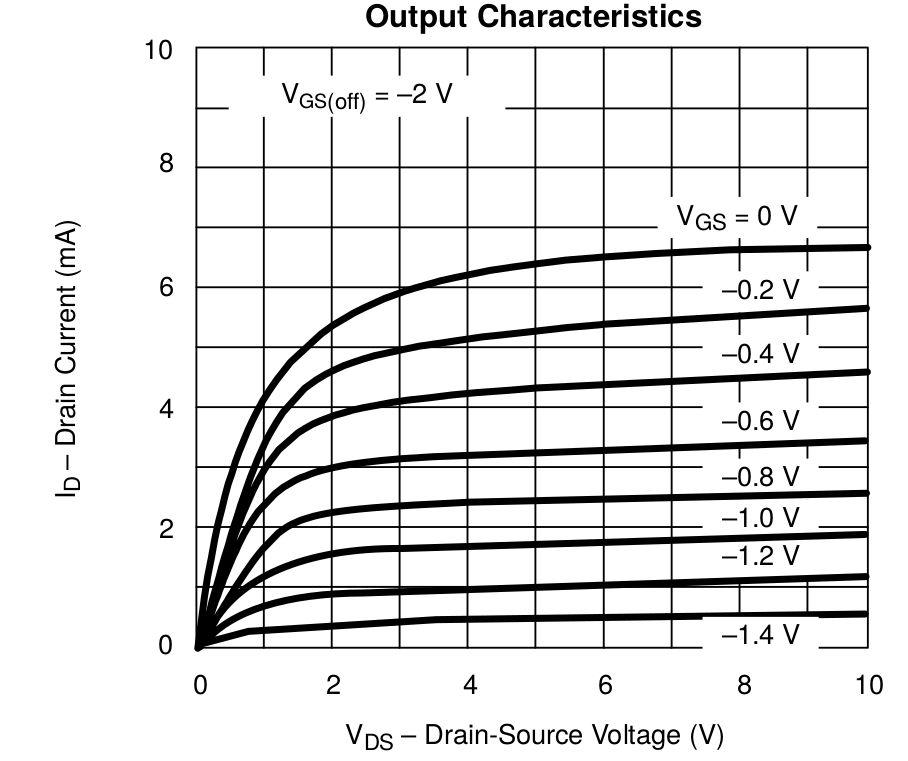
\includegraphics[scale=0.4]{char1.png}
\caption{Curve caratteristiche del JFET dal datasheet.\label{curveCaratteristiche}}
\end{figure}
Il grafico \ref{curveCaratteristiche} riporta un immagine delle curve caratteristiche del JFET nel caso in cui la tensione di \emph{pinch-off} sia $V_P = -2.0 V$, sul quale è riportata la retta di carico. Si vede che per i valori delle tensioni $V_{DS}$ esplorati (calcolati dalla retta di carico e riportati nella tabella \ref{correnteId} siamo semre in zona di saturazione. Dunque è possibile eseguire un fit di una funzione parabolica (togliendo i dati in cui siamo in interdizione) per stimare i parametri della legge empirica: $I_D = K_P (V_{GS} - V_P)^2$. Il punto del grafico per cui $V_{GS} = 0 V$ corrisponde alla corrente $I_{DSS}$, alternativamente si possono utilizzare le informazioni del fit: $I_{DSS} = K_P V_{P}^2$. I due valori sono compatibili entro l'errore. Il valore di $V_P$ è molto variabile per costruzione, ma il valore misurato è compatibile con il \emph{range} indicato nel datasheet \rem{dire quale...}. 


\paragraph{Stima della tensione $V_P$ e della corrente $I_DSS$}

\section{Montaggio amplificatore}

\section{Misure a frequenza fissa}
\section{Misura impedenza di ingresso}
\section{Aumento del guadagno}



\end{document}